\documentclass[10pt,twocolumn, nofootinbib]{revtex4-1}
%\documentclass[aps,pra,10pt,twocolumn,floatfix,nofootinbib]{revtex4-1}
%\documentclass[10pt,twocolumn,letterpaper]{article}

% Math packages
\usepackage{amsthm}
\usepackage{amsmath}
\usepackage{amssymb}

% For more complicated table formatting
\usepackage{multirow}
\usepackage{tabularx}
\newcolumntype{L}[1]{>{\raggedright\let\newline\\\arraybackslash\hspace{0pt}}m{#1}}
\newcolumntype{C}[1]{>{\centering\let\newline\\\arraybackslash\hspace{0pt}}m{#1}}
\newcolumntype{R}[1]{>{\raggedleft\let\newline\\\arraybackslash\hspace{0pt}}m{#1}}

% Remove line spaces between items of enumerate and itemize
\usepackage{enumitem}
\setlist{noitemsep}

% Adds double bracket symbols
\usepackage{stmaryrd}

% Allows to create negation symbols
\usepackage{MnSymbol}

% General math symbols
\DeclareMathOperator{\Id}{Id} % Identity function

% LOGIC symbols
% -------------

% Boolean symbols and algebra
\def\Bool{\mathbb{B}}
\def\TRUE{\textsc{true}}
\def\FALSE{\textsc{false}}
\def\AND{\wedge}
\def\bigAND{\bigwedge}
\def\OR{\vee}
\def\bigOR{\bigvee}
\def\NOT{\neg}

% Logical context and related symbols
\def\logCtx{\mathcal{S}}
\def\vstmtSet{\mathcal{S}_\textsf{v}}
\def\dstmtSet{\mathcal{S}_\textsf{d}}
\newcommand{\pAss}[1][\mathcal{S}] {\mathcal{A}_{#1}}
\DeclareMathOperator{\truth}{truth}

% Experimental test symbols
\newcommand{\exptSet}{\mathcal{E}}
\newcommand{\expt}[1][e] {\mathsf{#1}}
\DeclareMathOperator{\result}{result}
\def\SUCCESS{\textsc{success}}
\def\FAILURE{\textsc{failure}}
\def\UNDEF{\textsc{undefined}}

% Statements
\def\tautology{\top} % Tautology
\def\contradiction{\bot} % Contradiction
\newcommand{\stmt}[1][s] {\mathsf{#1}} % Statement
\newcommand{\tstmt}[1][s] {\bar{\mathsf{#1}}} % Theoretical statement

% Relationships between statements
\def\comp{\doublefrown} % Compatibility
\def\ncomp{\ndoublefrown} 
\def\narrower{\preccurlyeq} % Narrowness
\def\nnarrower{\npreccurlyeq}
\def\snarrower{\prec}
\def\nsnarrower{\nprec}
\def\broader{\succcurlyeq} % Broadness
\def\nbroader{\nsucccurlyeq}
\def\sbroader{\succ}
\def\nsbroader{\nsucc}
\def\indep{\upmodels} % Independent
\def\nindep{\nupmodels}

% Experimental domains and related symbols
\newcommand{\edomain}[1][D] {\mathcal{#1}} % Experimental domain
\newcommand{\tdomain}[1][D] {\bar{\mathcal{#1}}} % Theoretical domain
\newcommand{\basis}[1][B] {\mathcal{#1}} % Basis
\newcommand{\resPoss}[1][x] {\mathring{#1}} % Residual possibility
\newcommand{\estPoss}[1][x] {\dot{#1}} % Established possibility

% Formatting for experimental relationships
\newcommand{\erel}[1][r] {#1}

% Formatting for sentence statements
\newcommand{\statement}[1] {\emph{``#1"}}

% Formatting for reference
\newcommand{\refStmt}[1][r]{\textbf{#1}}

\DeclareMathOperator{\ver}{ver}
\DeclareMathOperator{\fal}{fal}
\DeclareMathOperator{\und}{und}

\DeclareMathOperator{\interior}{int}
\DeclareMathOperator{\exterior}{ext}

% Level of detail
\def\eqgran{\doteq}
\def\finer{\leqdot}
\def\nfiner{\nleqdot}
\def\coarser{\geqdot}
\def\sfiner{\lessdot}
\def\scoarser{\gtrdot}

% Theorem styles

%\renewcommand\thesubsection{\thesection.\Alph{subsection}}
%\renewcommand{\theequation}{\thechapter.\arabic{equation}}

\newtheorem{assump}{Assumption}
\renewcommand*{\theassump}{\Roman{assump}}

\newtheorem{axiom}[equation]{Axiom}
\newtheorem{defn}[equation]{Definition}
\newtheorem{prop}[equation]{Proposition}
\newtheorem{coro}[equation]{Corollary}
\newtheorem{thrm}[equation]{Theorem}

%\theoremstyle{definition}

\newenvironment{remark}{\emph{Remark}.}{}
\newenvironment{rationale}{\emph{Rationale}.}{\qed}
\newenvironment{justification}{\emph{Justification}.}{\qed}
\renewenvironment{proof}{\emph{Proof}.}{\qed}



\usepackage{graphicx}
\usepackage{hyperref}
\hypersetup{
	colorlinks=true,
	citecolor=blue,
	urlcolor=blue,
	linkcolor=blue
}
\urlstyle{same}
\frenchspacing


\begin{document}

\title{Assumptions of Physics overview: \\
	experimental verifiability and topology }
\author{Gabriele Carcassi, Christine A. Aidala}
\affiliation{Physics Department, University of Michigan, Ann Arbor, MI 48109}

\date{\today}


\begin{abstract}
We briefly show how the use of topological spaces and $\sigma$-algebras in physics can be rederived and understood as the fundamental requirement of experimental verifiability. A set of experimentally distinguishable objects will necessarily be endowed with a topology that is Kolmogorov (i.e. $T_0$) and second countable, which puts severe constrains on the space of well-formed scientific theories. These idea can be taken as a first step in a general mathematical theory for experimental science. This work is an overview of some of the results of Assumptions of Physics, a project that aims to identify a handful of physical principles from which the basic laws can be rigorously derived  (\url{https://assumptionsofphysics.org}).
\end{abstract}

\maketitle

\section{Introduction}

The overall structure (see \cite{AoPBook} for more details) can be summed up in the following diagram that can be used as a guide throughout this note.

\begin{figure}[h]
	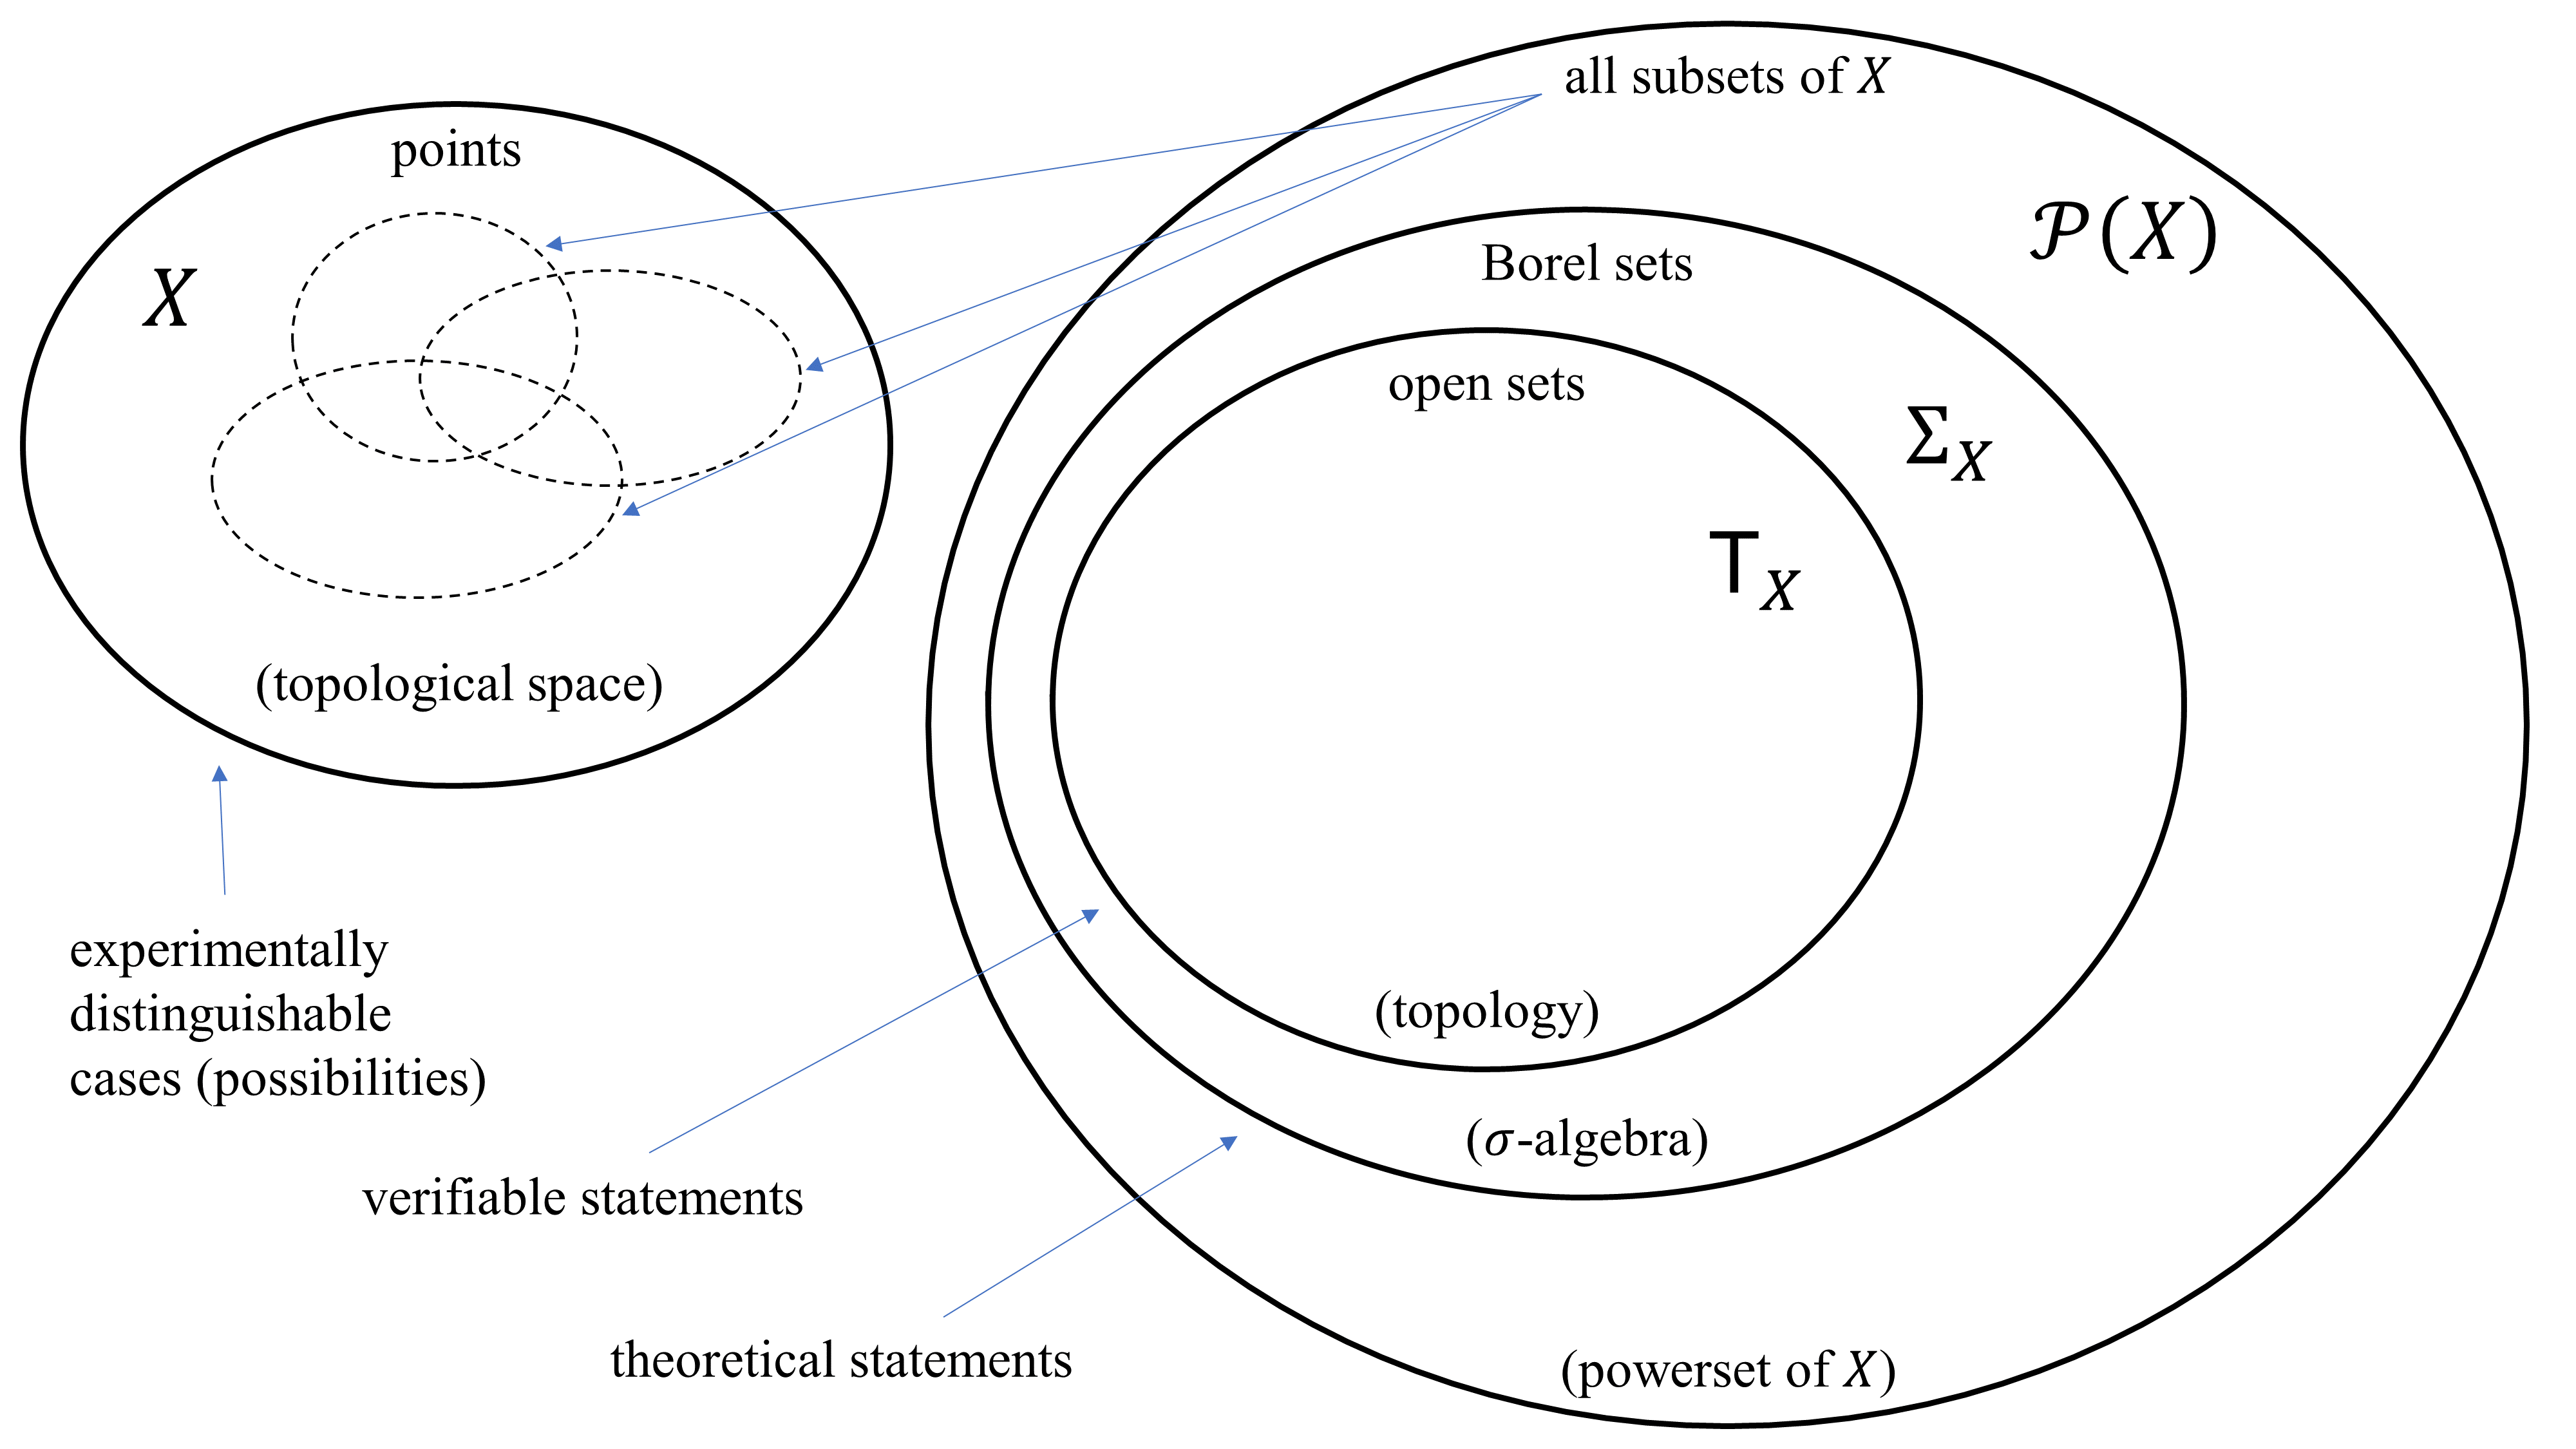
\includegraphics[width=\columnwidth]{Diagram.png}
\end{figure}

The set of points of a topological space represent the possible cases (e.g. all possible values for the mass of a particle). Each element in the topology (i.e. each open set) represents a statement that can be experimentally verified (e.g. the mass of the particle is within a finite precision interval). Each element in the Borel algebra represent a statement that, though it may or may not be experimentally verified, is sound within the theory (e.g. the mass of the particle is exactly zero, the mass of the particle is an irrational number). The Assumptions of Physics framework rederives this structure from the idea that a scientific theory must be logically consistent and evidence based.

\section{Logical context and fundamental axioms}

The guiding principle is that \emph{science is universal, non-contradictory and evidence based.} This means that any scientific theory must specify a set of \textbf{statements} that are logically consistent, whose truth can be confirmed experimentally by everybody. This starting point is codified in the axioms that form the formal foundation of the theory. We start with the axioms of logic.

The \emph{axiom of context} tells us that statements are organized into a \textbf{logical context} $\logCtx$, and a well defined truth value for each statement must exist. This recognizes that the logical consistency and meaning of each statement depends on definitions and relationships that depends on the context, on a set of statements.\footnote{For example, if one is performing particle identification, the mass of an electron is assumed to be given. If one is measuring the mass, the identify is assumed to be given, which the value of the mass is unknown.}

The \emph{axiom of possibility} tell us that the statements in a context cannot be assigned arbitrary truth values, but only in a way that is consistent with the meaning defined by the context.\footnote{For example, \statement{the mass of the object is one kilogram} and \statement{the mass of the object is two kilograms} cannot be both true.} Therefore each context comes with a set $\pAss$ of possible assignments, where each possible assignment is a function $a : \logCtx \to \Bool$ that returns a value of truth for each statement. The truth is a possible assignment.

The \emph{axiom of closure} tells us that we can always find a statements whose truth arbitrarily depends on the truth of other statements.

From the logic axioms one can show that each logical context is a complete Boolean algebra; that the narroness operator $\narrower$ that tells us whether a statement is more specific than another\footnote{For example, \statement{the mass of the object is between 4 and 5 kilograms} is narrower than \statement{the mass of the object is between 0 and 100 kilograms}.} provides a partial order for the context; that we can define intuitive relationship between statements, such as compatibility or independence.

Next, we introduce the axioms of verifiable logic. The \emph{axiom of verifiability} tells us that some statements are \textbf{verifiable}, meaning we have a test at our disposal that will terminate successfully in finite time if and only if the statement is true. Note that the test is not guaranteed to terminate, to give an answer, if the test is false.\footnote{For example, a test for \statement{there exists extra-terrestrial life} may terminate successfully if life is found, but it will not be conclusive if life is not found.} Therefore the negation of a verifiable statement is not necessarily verifiable.

The remaining two axioms tell us that the finite conjunction and the countable disjunction of verifiable statements is verifiable. That is, we can use the tests of the statement to construct the test for the logical AND (i.e. check that all tests terminates successfully) and the logical OR (i.e. check that at least one test terminates).

These axioms provide the ability to keep track the logical relationships between a set of statements and their connection to experimental evidence.

\section{Experimental and theoretical domains}



\section{Topologies and $\sigma$-algebras}

\section{Experimental relationships and continuous functions}

\bibliography{bibliography}


\end{document}